\chapter{Magnetismo de sólidos} \label{Ch:10}

En este Capítulo se estudian algunas de las contribuciones más importantes al magnetismo de los sólidos. Como se verá, alguna de ellas (como la ferromagnética) constituye un fenómeno cooperativo que lleva asociado una transición de fase. Es también destacable que el magnetismo de sólidos es en buena medida un efecto cuántico dado que muchas de sus causas (el momento mangnético de espín, la interacción de intercambio, etc.) no tienen análogo clásico.

\section{Relaciones básicas}

La \textbf{magnetización} (o imanación) $\Mn$ se define como el momento magnético por unidad de volumen 

\begin{equation}
	\Mn = \frac{1}{V} \sum_V \mun	
\end{equation}
donde los $\mun$ son los momentos magnéticos atómicos o iónicos en el ``volumen de control'' $V$. Recordemos que para partículas sin espín $\mun =  \sum_i \frac{1}{2} \rn_i \times q_i \vn_i$ y que para \textit{lazos} de corriente $\mun  = I \An$ siendo $I$ la intensidad y  $\An$ el área encerrada. El magnetismo de los sólidos se clasifica de acuerdo a la interrelación de su magnetización con el campo magnético aplicado $\Hn$. Así, se introduce la \textit{susceptibilidad magnética} $\chi$ por 

\begin{equation}
	\Mn = \chi \Hn
\end{equation}
En general $\chi$ será un tensor, pero no consideraremos esta complicación aquí. Si un medio tiene $\chi$ negativa se el sólido se dice \textit{diamagnético} y si por contra $\chi$ es positiva el sólido se dice \textit{paramagnético}. Además, existe un grupo de materiales que pueden poseer magnetización aun en ausencia de campo aplicado y que son \textit{ferromangéticos} (observar que $\chi \rightarrow \infty$).

\section{Diamagnetismo atómico}

La naturaleza del diamagnetismo atómico se puede comprender a partir de un modelo clásico en que cada órbita electrónica es considerada una espira de corriente. De acuerdo con la ley de Lenz, al variar el flujo magnético sobre el circuito surge una fuerza electromotriz de inducción que hace variar la corriente y por tanto genera un momento magnético adicional. Así, si $A$ es el área de la órbita, $\omega$ la velocidad angular e $I$ la intensidad de corriente, el momento magnético será $\mu=IA=-(e\omega / 2\pi)A$, y bajo la aplicación de un campo $B$ perpendicular a la órbita, aquél se incrementa en

\begin{equation}
	\Delta \mu = - \frac{eA}{2\pi} \Delta \Omega \label{Ec:10-02-01}
\end{equation}
La variación de velocidad angular $\Delta \omega$ se determina del balance de fuerzas sobre la órbita, que consideramos circular de radio $r$ (ver figura \ref{Fig:10-01}): antes de la aplicación del campo de fuerza nuclear se equipara a la fuerza centrífuga, $F_\text{núcleo} = m\omega^2 r$; tras la aplicación del campo aparece adicionalmente la fuerza de Lorentz $F_L = ev B$ dirigida hacia el núcleo, que se compensa con un aumento de la velocidad angular 

\begin{equation}
	m(\omega + \Delta \omega)^2 r = F_\text{núcleo} + e v B
\end{equation}
Como para los campos magnéticos aplicables en un laboratorio $evB\ll m \omega^2 r$, se tiene que $\Delta \omega \ll \omega$. Así pues, despreciando términos en $\Delta \omega^2$ se deduce 

\begin{equation}
	\Delta \omega = \frac{evB}{2mr\omega} = \frac{eB}{2m}
\end{equation}
que se denomina \textit{frecuencia de Larmor}. Combinando con (\ref{Ec:10-02-01}) y generalizando a un átomo de $Z$ electrones:

\begin{equation}
	\Delta \mu = - Z \frac{e^2A}{4\pi m} B = - Z \frac{e^2 \langle \rho^2 \rangle}{4m}B
\end{equation}
siendo $\langle \rho^2 \rangle = \langle x^2 + y^2 \rangle = \langle x^2 \rangle + \langle y^2 \rangle$ el valor cuadrático medio de la distancia de los electrones al eje que pasa por el núcleo paralelamente al campo (eje $z$). Si admitimos simetría esférica, $\langle x^2 \rangle=\langle y^2 \rangle=\langle z^2 \rangle$ y con ello el radio cuadrático medio atómico resulta $\langle r^2 \rangle = \frac{3}{2} \langle \rho^2 \rangle$. Llamando $n$ al número de átomos por unidad de volumen la magnetización resultante es

\begin{equation}
	M = n \Delta \mu = - \frac{nZe^2 \langle r^2 \rangle}{6m}B
\end{equation}
y la susceptibilidad magnética 

\begin{equation}
	\chi = \frac{M}{H} \approx \frac{mu_0 M}{B} = - \frac{\mu_0 n Z e^2 \langle r^2 \rangle}{6m}
\end{equation}
que es el resultado clásico de \textit{Langevin}. Aunque en general $B=\mu_0 (H+M)$, aquí se ha aproximado $B\approx \mu_0 H$ dado que $|M|\ll H$ (o bien que $|\chi |\ll 1$). En efecto, para $n=5\times10^{28} \unit{m}^{-3}$ y $r=10^{-10}$ m, $\chi = -10^{-6}Z$. El diamagnetismo atómico es propio de \textit{todos los cuerpos sin excepción}, aunque a menudo está enmascarado por el paramagnetismo o el ferromagnetismo.

\begin{figure}[h!] \centering
	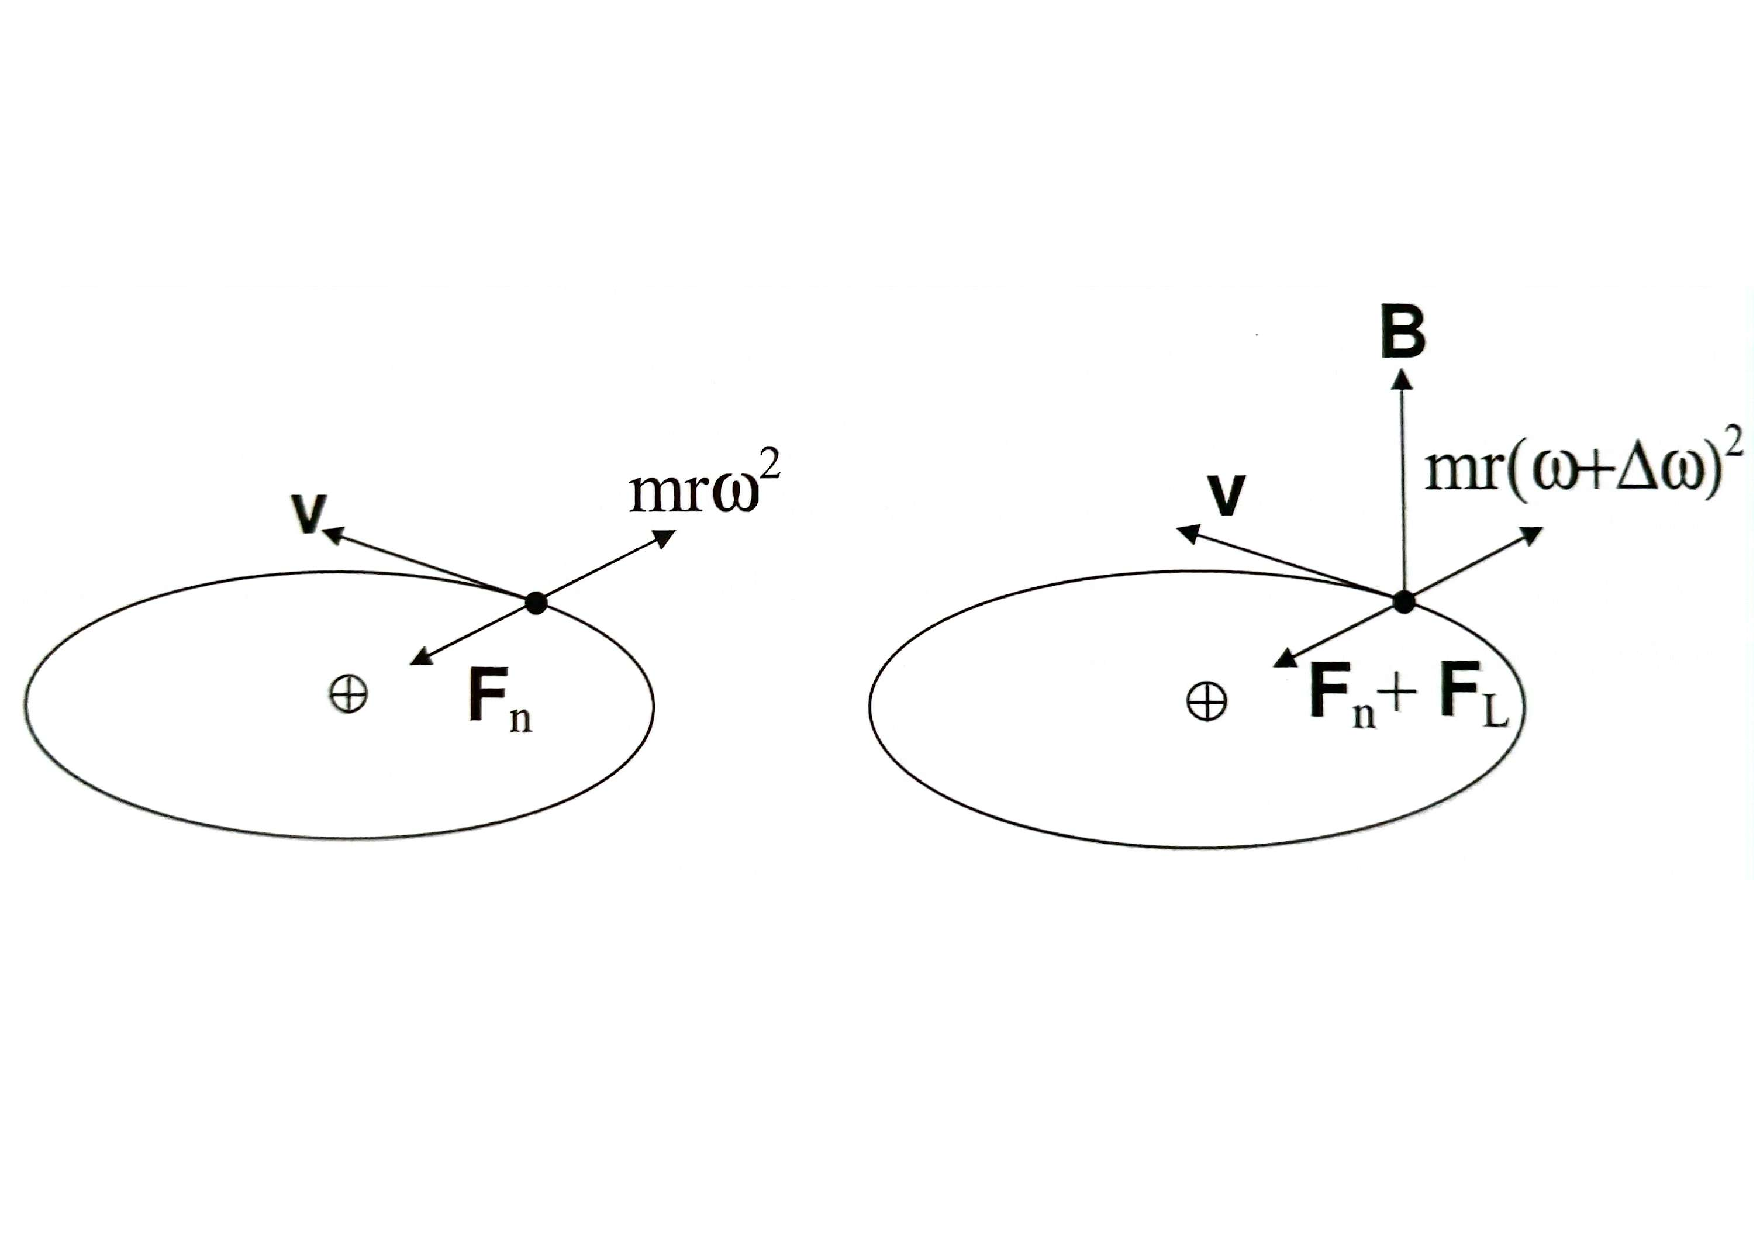
\includegraphics[scale=0.35]{Cuerpo/Ch_10/Fotos libro 1.pdf}
	\caption{Balance  de fuerzassobre un electrón orbitando en torno a un núcleo en ausencia (izquierda) o en presencia (derecha) de un campo mangético externo. El referencial usado es uno centrado en el núcleo y que gira con el electrón de modo qeu hay que considerar las fuerzas inerciales (aquí sólo hay fuerza centrífuga).}
	\label{Fig:10-01}
\end{figure}

\section{Paramagnetismo atómico}

Además de la contribución diamagnética ya vista en la sección anterior, algunos átomos presentan un momento magnético \textit{permanente} debido al espín y al momento angular orbital de los electrones (los momentos magnéticos nucleares son $\sim 10^3$ veces más pequeños y no se tendrán en cuenta). En ausencia de un campo externo los momentos magnéticos atómicos están orientados al azar y la magnetización resultante es nula. Sin embargo, como se verá, bajo la aplicación de un campo magnético los momentos atómicos se orientan en su mismo sentido dando lugar a una mangnetización (\textit{paramagnética}), que puede ser mucho mayor que la diamagnética.

\subsection{Origen del momento mangnético atómico}

El momento mangético orbital electrónico $\mun_L$ se relaciona con el momento angular orbital $\hbar \Ln$ por 

\begin{equation}
	\mun_L \equiv - \frac{e}{2m} \rn \times \pn = - \mun_B \Ln
\end{equation}
donde $\mu_B=e\hbar / 2m=9.3\times 10^{-24}$ J/T es el llamado \textit{magnetón de Bohr}. Los momentos magnéticos magnéticos de espín $\mun_S$ están relacionados con el momento angualr de espín $\hbar \Sn$ por:

\begin{equation}
	\mun_S = - g_0 \mu_B \Sn  \label{Ec:10-03-02}
\end{equation}
siendo $g_0 \approx 2$. Como para un solo electrón $S=1/2$, $\mu_B$ es interpetrable como el momento mangético de espín de un electrón libre. En el caso atómico (varios electrones con contribución orbital y de espín) el momento magnético total $\mun$  también resulta ser proporcional al momento angular electrónico total $\hbar\Jn=\hbar \Ln + \hbar \Sn$ según 

\begin{equation}
	\mun = - g \mu_B \Jn 
\end{equation}
donde 

\begin{equation}
	g = 1 + \frac{J(J+1)+S(S+1)-L(L-1)}{2J(J+1)}
\end{equation}
es el llamado \textit{factor de Landé}. El momento magnético asociado a átomos e iones con capas electrónicas cerradas es nulo. Si existen capas electrónicas interiores parcialmente desocupadas (elementos de transición, tierras raras y actínidos), o capas de valencia con número impar de electrones el momento magnético es distinto de cero. El cálculo de $L,S$ y $J$ del estado atómico fundamental a partir de los momentos angulares electrónicos individuales se hace por las reglas de Hund:

\begin{enumerate}
	\item $S$ toma el valor más alto posible compatible con el principio de exclusión (momentos magnéticos de espín paralelos).
	\item $L$  toma el máximo valor compatible con este valor de $S$ (momentos magnéticos paralelos).
	\item $J=|L-S|$ para una capa llena a menos de la mitad, y $J=L+S$ si a más de la mitad.
\end{enumerate}

\subsection[Dependencia de la magnetización respecto $\vec{\Bn}$ y $T$]{Dependencia de la magneteización paramagnética con la temperatura y el campo magnético}

Los niveles de energía de un momento magnético $\mun$ en un campo de inducción $\Bn$ en la dirección de $z$ se expresan por 

\begin{equation}
	U = - \mun \cdot \Bn = g \mu_B \Jn \cdot \Bn = g \mu_B J_z B \tquad \mu_z = g \mu_B J_z
\end{equation}
donde $J_z = - J_1,...,J$ es el \textit{número cuántico azimutal o magnético}. Queremos calcular el valor medio de $J_z$ (las componentes no paralelas al campo promedian a cero). Estadísticamente la ocupación relativa de niveles a temperatura $T$ la da el factor de Boltzmann $\exp (-U/k_B T)=\exp \parentesis{-g\mu_B J_z B / k_B T}$, de modo que la magnetización neta $M$ de un conjunto de momentos magnéticos \textit{independientes} con una concentración $n$ vendrá dada por 

\begin{equation}
	M = n \frac{\sum_{J_z=-J}^{+J} - g\mu_B J_z \exp \parentesis{- g\mu_B J_z B / k_BT}}{\sum_{J_z=-J}^{+J} \exp \parentesis{-g\mu_B J_z B / k_B T}} \label{Ec:10-03-06}
\end{equation}
tras algunas manipulaciones la suma anterior se iguala a 
\begin{mybox}
\begin{equation}
	M = n g \mu_B J B_J (x) \label{Ec:10-03-07}
\end{equation}
\end{mybox}
donde 

\begin{equation}
	B_J (x) = \frac{2J+1}{2J} \coth \parentesis{\frac{2J+1}{2J}x} - \frac{1}{2J} \coth \parentesis{\frac{x}{2J}} \quad x \equiv \frac{g\mu_B J B }{k_B T}
\end{equation}
es la \textbf{función de Brilluoin}. $B_J$ crece linealmente con $x$ para $x\ll 1$ y satura a q para valores altos de $x$. Por tanto $M$ tiene a la magneteización de saturación a campos $B$ altos correspondiendo al máximo alineamiento de los dipolos con el campo $J_z = -J$. La figura \ref{Fig:10-02} ilustra la variación de $B_J(x)$ y de la magnetización paramagnética para distintos $J$.

\begin{figure}[h!] \centering
	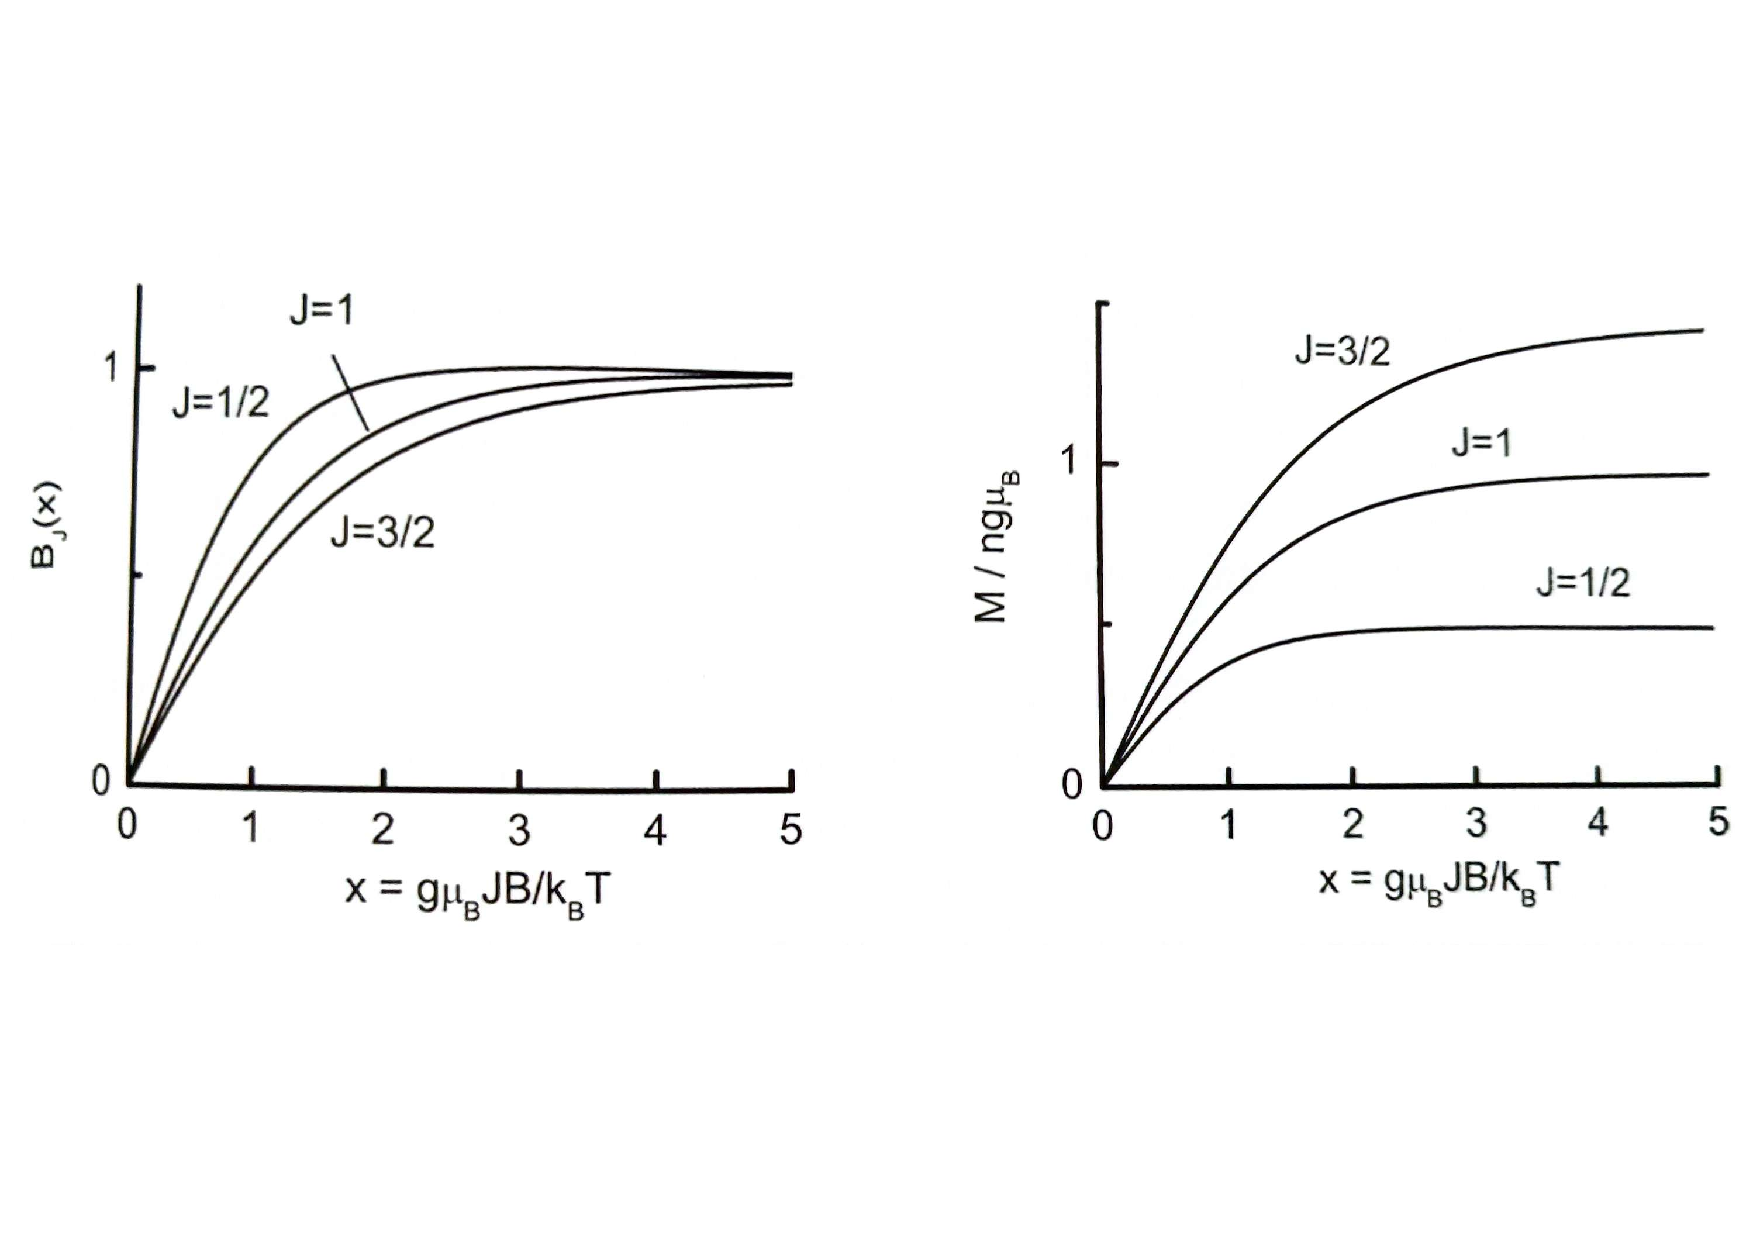
\includegraphics[scale=0.35]{Cuerpo/Ch_10/Fotos libro 2.pdf}
	\caption{Dependencia con $x$ de la función de Brillouin y de la magnetización paramagnética para distintos valores de $J$.}
	\label{Fig:10-02}
\end{figure}

\subsection{Ley de Curie}

A temperatura ambiene, para los campos más altos alcanzables en un laboratorio $(\sim 10$ T) $x\ll 1$, y $B_J(x)$ se aproxima Por

\begin{equation}
	B_J (x) = \frac{J+1}{3J} x
\end{equation}
de modo que la susceptibilidad paramangética es 

\begin{equation}
	\chi = \frac{M}{H} \approx \frac{mu_0 M}{B} = \frac{nJ(J+1)g^2 \mu_0 mu_B^2}{3k_BT} \label{Ec:10-03-11}
\end{equation}
donde $p=g \sqrt{J(J+1)}$ es el \textit{número efectivo de magnetos de Bohr}. La relación (\ref{Ec:10-03-11}) se denomina \textbf{ley de Curie} y a $C$ se le denomina \textit{constante de Curie}. Numéricamente se encuentra que $\chi\sim 10^{-3}$, lo que justifica la aproximación $B=\mu_0 (H+M) \approx \mu_0 H$. Es destacable que, aunque pequeña, es $10^2-10^3$ veces mayor que la correspondiente a la contribución diamangética.

% tabla 

La tabla muestra la comparación entre el valor de $p$ teórico y el experimental determinado por el coeficiente en $1/T$ de la susceptibilidad medida para un conjunto de iones de tierras raras (capa $f$ interna incompleta). El acuerdo es muy  bueno excepto para el Eu para el que como $J=0$, habría que que considerar la contribución a $M$ en (\ref{Ec:10-03-06}) de otros multipletes (estados excitados con distinto $J$). La situación es muy distinta para los iones de los elementos de transición (capa $d$ externa incompleta), como se muestra en la tabla , donde aunque se verifica la ley de Curie sólo hay acuerdo si se admite que $L=0$. Se interpreta esta anulación del momento angular orbital como un efecto producido por los iones vecinos, siendo afectadas las capas electrónicas $d$ por el campo eléctrico que estos generan (a esto lo llamamos \textit{efecto de campo cristalino}). Éste, sin embargo, no afecta a las tierras raras pues la capa interna $f$ está mucho más cerca del núcleo y protegida del campo ``ambiental'' por las capas $5s$ y $5p$.

% tabla

\section{Paramagnetismo de los electrones de conducción}

Los resultados anteriores no son válidos para los electrones de conducción pues por el principio de exclusión no se pueden considerar independientes, que es lo que hemos admitido en la sección anterior. En efecto, vamos a ver cómo el principio de Pauli limita fuertemente el alineamiento de los espines electrónicos con el campo. La figura \ref{Fig:10-03} muestra cómo actúa un campo magnético $B$ sobre el mar de Fermi.

\begin{figure}[h!] \centering
	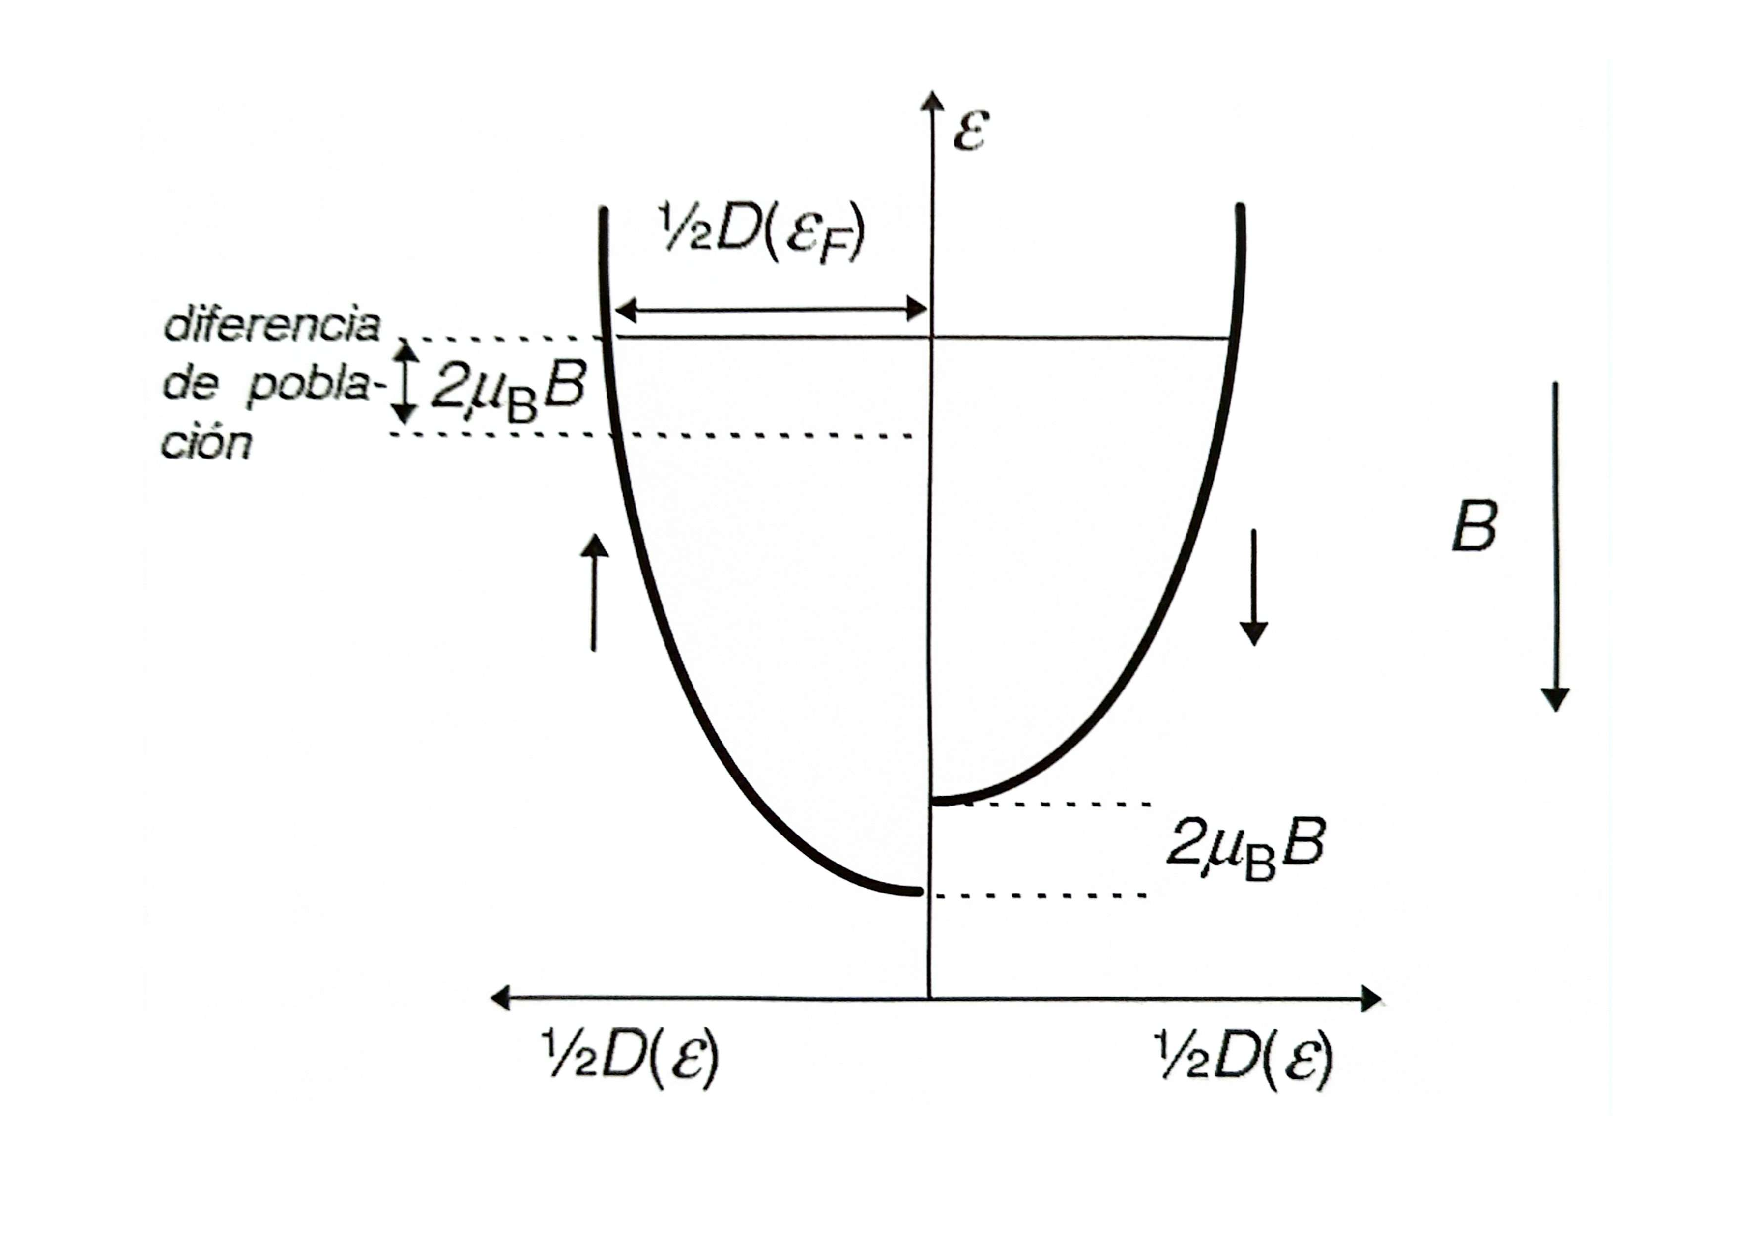
\includegraphics[scale=0.35]{Cuerpo/Ch_10/Fotos libro 3.pdf}
	\caption{Desplazamiento relativo de los niveles energéticos electrónicos correspondientes a espín $\uparrow$ y espín $\downarrow$.}
	\label{Fig:10-03}
\end{figure}

Como $S=\pm 1/2$, por (\ref{Ec:10-03-02}) se tiene $\mu=\mu_B$, de modo que las energías electrónicas se corren en $\pm \mu_B B$ según la orientación del momento magnético de espín. La diferencia en la concentración de electrones con espín $\uparrow$ y $\downarrow$, $\Delta n$, es igual al área de la proporción rectangular indicada (observar también que la condición de equilibrio exige que el potencial químico $\varepsilon_F$ sea el mismo para ambos grupos de espines). Como para los mayores campos alcanzables $\mu_B B \ll \varepsilon_F$ (por ejemplo, $\mu_B B \approx 0.6 $ meV a $B=10$ T), el área se aproxima por $\Delta n \approx \frac{1}{2} D (\varepsilon_F) 2 \mu_B B$. Utilizando que para electrones libres $D(\varepsilon_F) = 3n/2\varepsilon_F = 3n/2k_B T_F$ resulta 

\begin{equation}
	M= \mu_B \Delta n = \frac{3n\mu_B^2}{2k_B T_F} B
\end{equation}
que se conoce como magnetización de espín de Pauli. Aquí se ha considerado que el mar de Fermi estaba completamente lleno, es decir, $T=0$ K. 

Landau mostró que se debe considerar la alteración del movimiento estapcial electrónico por el campo magnético, qeu da lugar a una contribución diamagnética igual a $-1/3$ de la paramagnética, de modo que finalmente:

\begin{equation}
	M = \frac{n\mu_B}{k_B T_F} B
\end{equation}
Numéricamente resulta una suscetibilidad $\sim 10^{-5}$; este valor concuerda dentro de un factor 2 para los metales alcalinos y es bastante inferior al experimental en algunos metales de transición debido a la contribución de los electrones $3d$ (además de los $4s$). Como la suscetibilidad paramagnética electrónica es sólo poco mayor que la diamagnética atómica (capas electrónicas internas) bastantes metales como el Al, Pb, Sb, Au, Zn, etc. resultan ser globalmente diamagnéticos.


\section{La interacción de intercambio}

La magnetización espontánea en ausencia de campo, propia de los materiales ferromangéticos es debida al alineamineto de los dipolos magnéticos (localizados o deslocalizados). La interacción magnética clásica entre dipolos es demasiado pequeña como para dar cuenta de este alinieamiento. En efecto, la energía de interacción de dos momentos magnéticos de magnitud $\mu_B$ a distancia $r=3\unit{\Angstrom}$ es $\mu_B^2 \mu_0 / 4\pi r^3 \approx 2 \times 10^{-6} $ eV, que en temperatura $k_BT$ tendríamos que $T\approx 0.03$ K, y sin embargo muchos materiales ferromagnéticos mantienen su magnetización espontánea a temperaturas del orden de 1000K. Vamos a ver cualitativamente que el orden del orden magnético reside paradojicamente en la interacción eléctrica entre electrones (orientación colectiva de espines).

Si consideramos dos electrones sabemos que la función de onda debe ser antisimétrica bajo permutación de coordenadas y espín $\Psi(\rn_1,\sn_1,\rn_2,\sn_2) = -\Psi(\rn_2,\sn_2,\rn_1,\sn_1)$, de donde se deduce que $\Psi=0$ para $\rn_1 = \rn_2$ y $\sn_1=\sn_2$. Esto no indica sino que para espines paralelos hay probabilidad nula de encontrar los dos electrones en la misma posición, pero no excluye dos electrones con espines opuestos. Así, la antisimietría de la función de odna tiende a mantener a los electrones con espines paralelos alejados y en consecuencia disminuye la energía de repulsión de Coulomb respecto la configuración de espines antiparalelos. Esto es lo que se conoce como \textbf{interacción de intercambio}. En caso de electrones atómicos, si se tienen en cuenta las energías electrostáticas de interacción con los núcleos puede ocurrir que a la distribución de carga orbital asociada a espines antiparaleos corresponda menor energía de modo que al final la interacción de intercambio favorece el antialineamiento.

Las dos situaciones opuestas se recogen en el llamado \textbf{modelo de Heisenberg}, en el cual la energía de interacción entre los átomos $i$ y $j$ está contenida en el término $\Jcal_{ij}$ tal que 

\begin{equation}
	U_{ij} = - \Jcal_{ij} \Sn_i \cdot \Sn_j
\end{equation}
donde $\Jcal$ es la llamada \textbf{integral de intercambio}, relacionada con el solapamiento de las distribuciones de carga de los átomos $i$ y $j$, que puede ser positiva o negativa. El hamiltoniano global sería:

\begin{equation}
	\Hcal = - \sum_{ij} \Jcal_{ij} \Sn_i \cdot \Sn_j
\end{equation}

\section{Ferromagnetismo}

Podríamos ahora definr un medio ferromagnético como aquél en el que existe una interacción de intercambio con integral de intercambio positiva, causando el alineamiento de espines origen de magnetización espontánea. Para simplificar el tratamiento que origina el término $U_{ij}$ se introduce la llamada \textit{aproximación de campo medio}: se supone que el efecto de interacción de canje de un espín $\Sn_i$ con otro $\Sn_j$ se puede calcular reemplazando $\Sn_j$ con su valor medio $\langle \Sn_j \rangle$. En ese caso, en un campo externo $\Bn$

\begin{equation}
	\Hcal = - \sum_{i,j} \Jcal_{ij} \Sn_i \cdot \Sn_j + g\mu_B \Bn \sum_i \Sn_i
\end{equation}
pasa a ser 
\begin{equation}
	\Hcal = - \sum_{i} \Sn_i \parentesis{ \sum_j \Jcal \langle \Sn_j \rangle g\mu_B \Bn \sum_i \Sn_i}
\end{equation}
En un medio homogéneo $\langle \Sn_j \rangle$ es el mismo para todos los espines. El valor común $\langle \Sn \rangle$ se relaciona con la magnetización por

\begin{equation}
	\Mn = - g \mu_B n \langle \Sn \rangle
\end{equation}
Además la suma $\sum_j \Jcal_{ij} \approx z \Jcal$ donde $z$ es el número de vecinos más próximos. Así:

\begin{equation}
	\Hcal = g \mu_B \parentesis{\frac{z\Jcal}{ng^2\mu_B^2}\Mn + \Bn} \cdot \sum_i \Sn_i
\end{equation}
Observar que esta es la energía que tendría un conjunto de espines desacoplados en presencia de un \textit{campo efectivo}

\begin{equation}
	\Bn_{\text{eff}} = \frac{z\Jcal}{ng^2\mu_B^2}\Mn + \Bn
\end{equation}
y si $\lambda = \frac{z\Jcal}{ng^2\mu_B^2\mu_0}$ tenemos que

\begin{equation}
	\Bn_{\text{eff}} = \lambda \mu_0\Mn + \Bn
\end{equation}
Dado que bajo $	\Bn_{\text{eff}} $ los espines se comportan como paramagnéticos, vamos a utilizar la ecuación anterior en los resultados anteriores del paramagnetismo para calcular la respuesta del material ferromagnético. Por ejemplo, a altas temperaturas, la susceptibilidad magnética puede aproximarse por

\begin{equation}
	\mu_0 \Mn = \chi_p \Bn_{\text{eff}}  = \lambda \mu_0\Mn + \Bn
\end{equation}
donde $\chi_p=C/T$ es la ley de Curie. Despejando $\Mn$ e introduciendo la \textit{temperatura de Curie} $T_c \equiv C\lambda$ tenemos que

\begin{equation}
	\mu_0 \Mn = \frac{C}{T-T_c} \Bn
\end{equation}
con lo que finalmente se tiene la susceptibilidad magnética efectiva
\begin{mybox}
\begin{equation}
	\chi = \frac{M}{H} \approx \mu_0 \frac{M}{B} = \frac{C}{T-T_c}
	\label{Ec:10-06-09}
\end{equation}
\end{mybox}
De nuevo, se ha utilizado $B\approx \mu_0 H$ dado que $\chi \ll 1$ salvo cuando $T\rightarrow T_c$ (donde $\chi\rightarrow \infty$). $T_c$ es la \textbf{temperatura de Cuerie}, y la fórmula anterior (\ref{Ec:10-06-09}) se llama la \textbf{ley de Curie-Weiss}, describiendo correctamente la susceptibilidad observada para $T>T_c$. 

Para ver lo que ocurre a $T<T_c$ hay que utilizar la expresión general (\ref{Ec:10-03-07}). Poniendo, por ejemplo, $J=1/2$, $S=1/2$ y $L=0$ ($g=2$) obtenemos que

\begin{equation}
	M = n \mu_B \tanh \parentesis{\frac{\mu_B B_{\text{eff}}}{k_B T}}
\end{equation}
Teniendo en cuenta que $\Bn_{\text{eff}} \approx \lambda \mu_0 \Mn$ e introduciendo las \textit{magnetización y temperatura reducidas}:

\begin{equation}
	m \equiv \frac{M}{n\mu_B} \tquad t \equiv \frac{T}{T_c}
\end{equation}
resulta 

\begin{equation}
	m = \tanh \parentesis{\frac{m}{t}} \Longrightarrow t = \frac{m}{\arctanh (m) } = \frac{2m}{\ln \ccorchetes{(1+m)/(1-m)}}
\end{equation}
La anterior ecuación sólo tiene solución para $t<1$, o sea $T<T_c$ de modo que $T_c$ marca la temperatura por debajo de la cual puede haber magnetización espontánea. Podríamos decir que para $T<T-c$ tenemos una fase ordenada (espines alineadas) y esta propiedad la que hace que el ferromagnetismo sea una transición de fase, y que $T_c$ su temperatura crítica. Cuando $T\rightarrow 0$, la imanación de saturación (todos los espines alineados) tiende a $M_s(0) = n \mu_B$ (en general a $ng\mu_B J$ si $J\neq 1/2$). Los datos experimentales refrendan aproximadamente el enfoque de campo medio como en la figura \ref{Fig:10-04}.

\begin{figure}[h!] \centering
	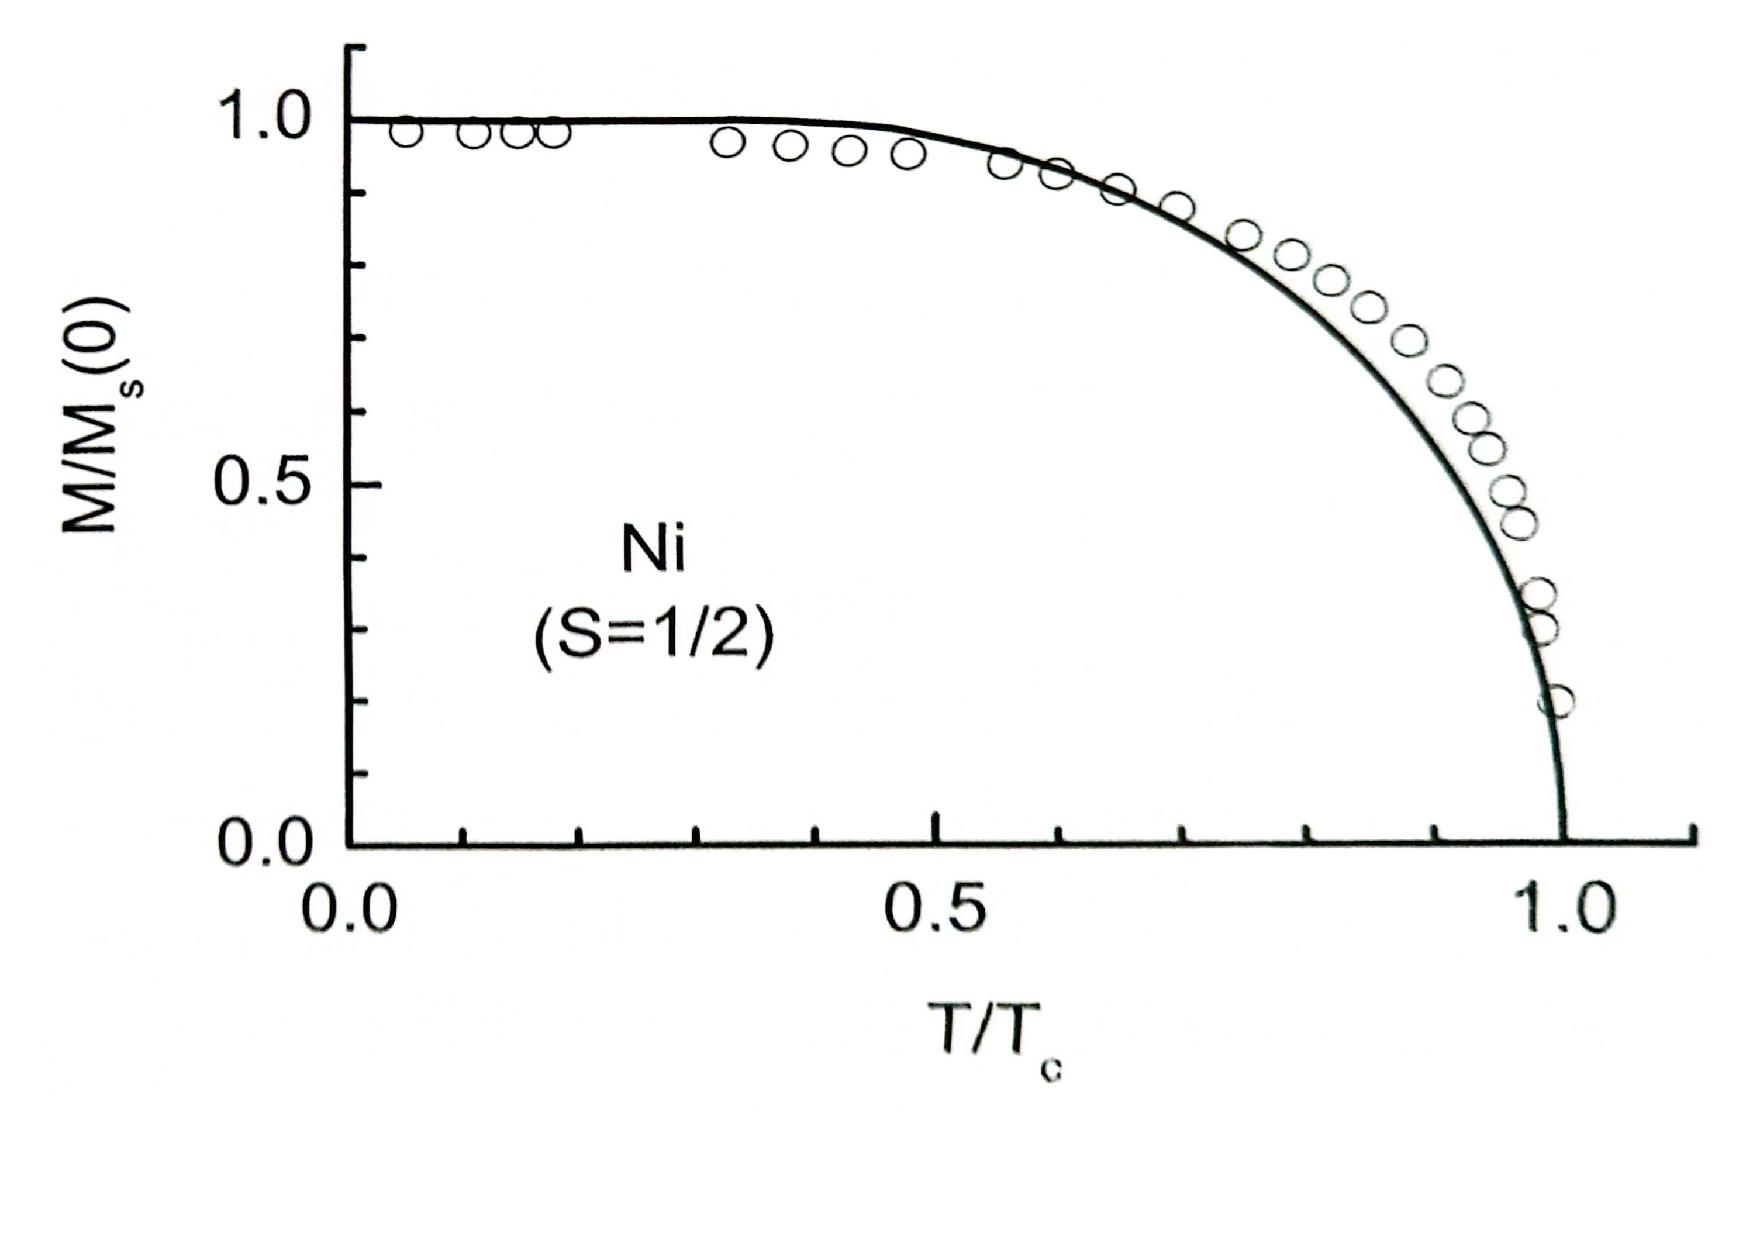
\includegraphics[scale=0.35]{Cuerpo/Ch_10/Fotos libro 4.pdf}
	\caption{Dependencia con la temperatura de la magnetización espontánea para el Ni cuando $T<T_C$, y compensación con las predicciones de campo medio.}
	\label{Fig:10-04}
\end{figure}

Experimentalmente se encuentra que $M_s(0) = n_B n \mu_B$ donde $n_B$ es el \textbf{número efectivo de magnetones de Bohr}. Hay que tener en cuenta que $n_B$ no siempre coincide con $gJ$. En particular para los metales de transición no coincide con $g_0S$. Para estos metales debe considerase un modelo de electrones itinerantes o de bandas, según el cual el magnetismo proviene del espín de los electrones de conducción pero por el desplazamiento relativa de las subbandas con espín arriba y abajo forzado por la interacción de intercambio.

\section{Dominios ferromagnéticos}

Aunque en una muestra ferromagnética a $T\ll T_c$ todos los momentos magnéticos son paralelos, a escala macroscópicas el momento mangético global peude ser mucho menor que el de saturación. La razón está en que las muestras se componen de pequeñas regiones llamadas \textit{dominios}, dentro de los cuales la magnetización está saturada pero la orientación puede variar de dominio a dominio. La existencia de dominios tiene su origen en el concurso de varias energías:

\begin{enumerate}[label=\alph*)]
	\item \textbf{Energía de anisotropía.} Ocurre que en los cristales se dan direcciones (o ejes) privilegiados o de fácil imanación y otras de difícil imanación. La causa de la anisotropía está en que por el acoplamiento espín-órbita una rotación de espín arrastra a la distribución de carga o parte orbital. Este hecho cambia la energía de canje entre espiens así como la energía electroestática de las distribuciones de carga entre átomos (distinto solapamiento etc.). Por ejemplo, en el cobalto, de estructura hexagonal, la densidad de energía de anisotropía se expresa por 
	
	\begin{equation*}
		u = K_1 \sin^2 \theta + K_2 \sin^4 \theta
	\end{equation*}
	donde $\theta$ es el ángulo de la magnetización con el eje hexagonal.
	
	\begin{figure}[h!] \centering
		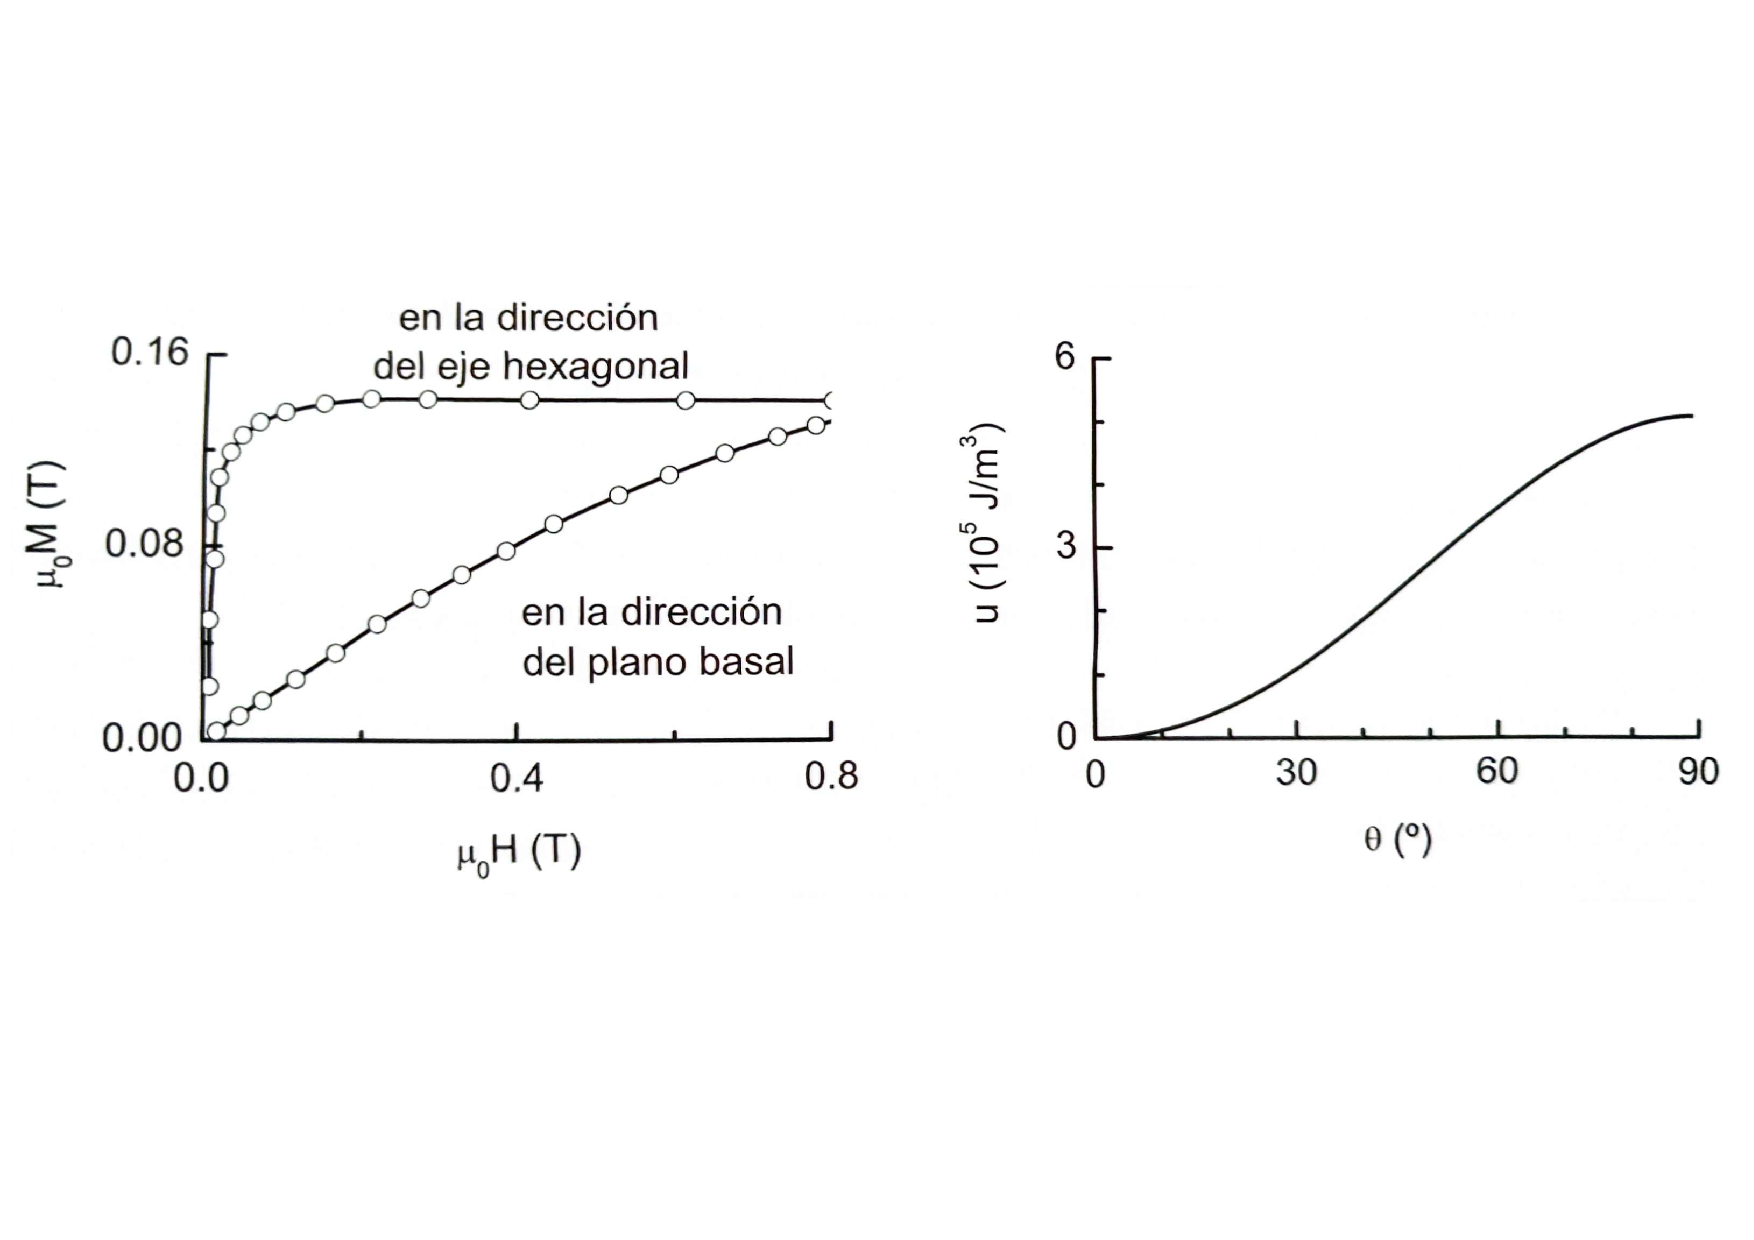
\includegraphics[scale=0.35]{Cuerpo/Ch_10/Fotos libro 5.pdf}
		\caption{En la izquierda la magnetización de una muestra de  Co para las direcciones paralela y perpendicular al plano basal de la estructura hexagonal. En la derecha de anisotropía del Co según el ángulo que forma la magnetización con el eje hexagonal.}
		\label{Fig:10-05}
	\end{figure}
	\begin{figure}[h!] \centering
	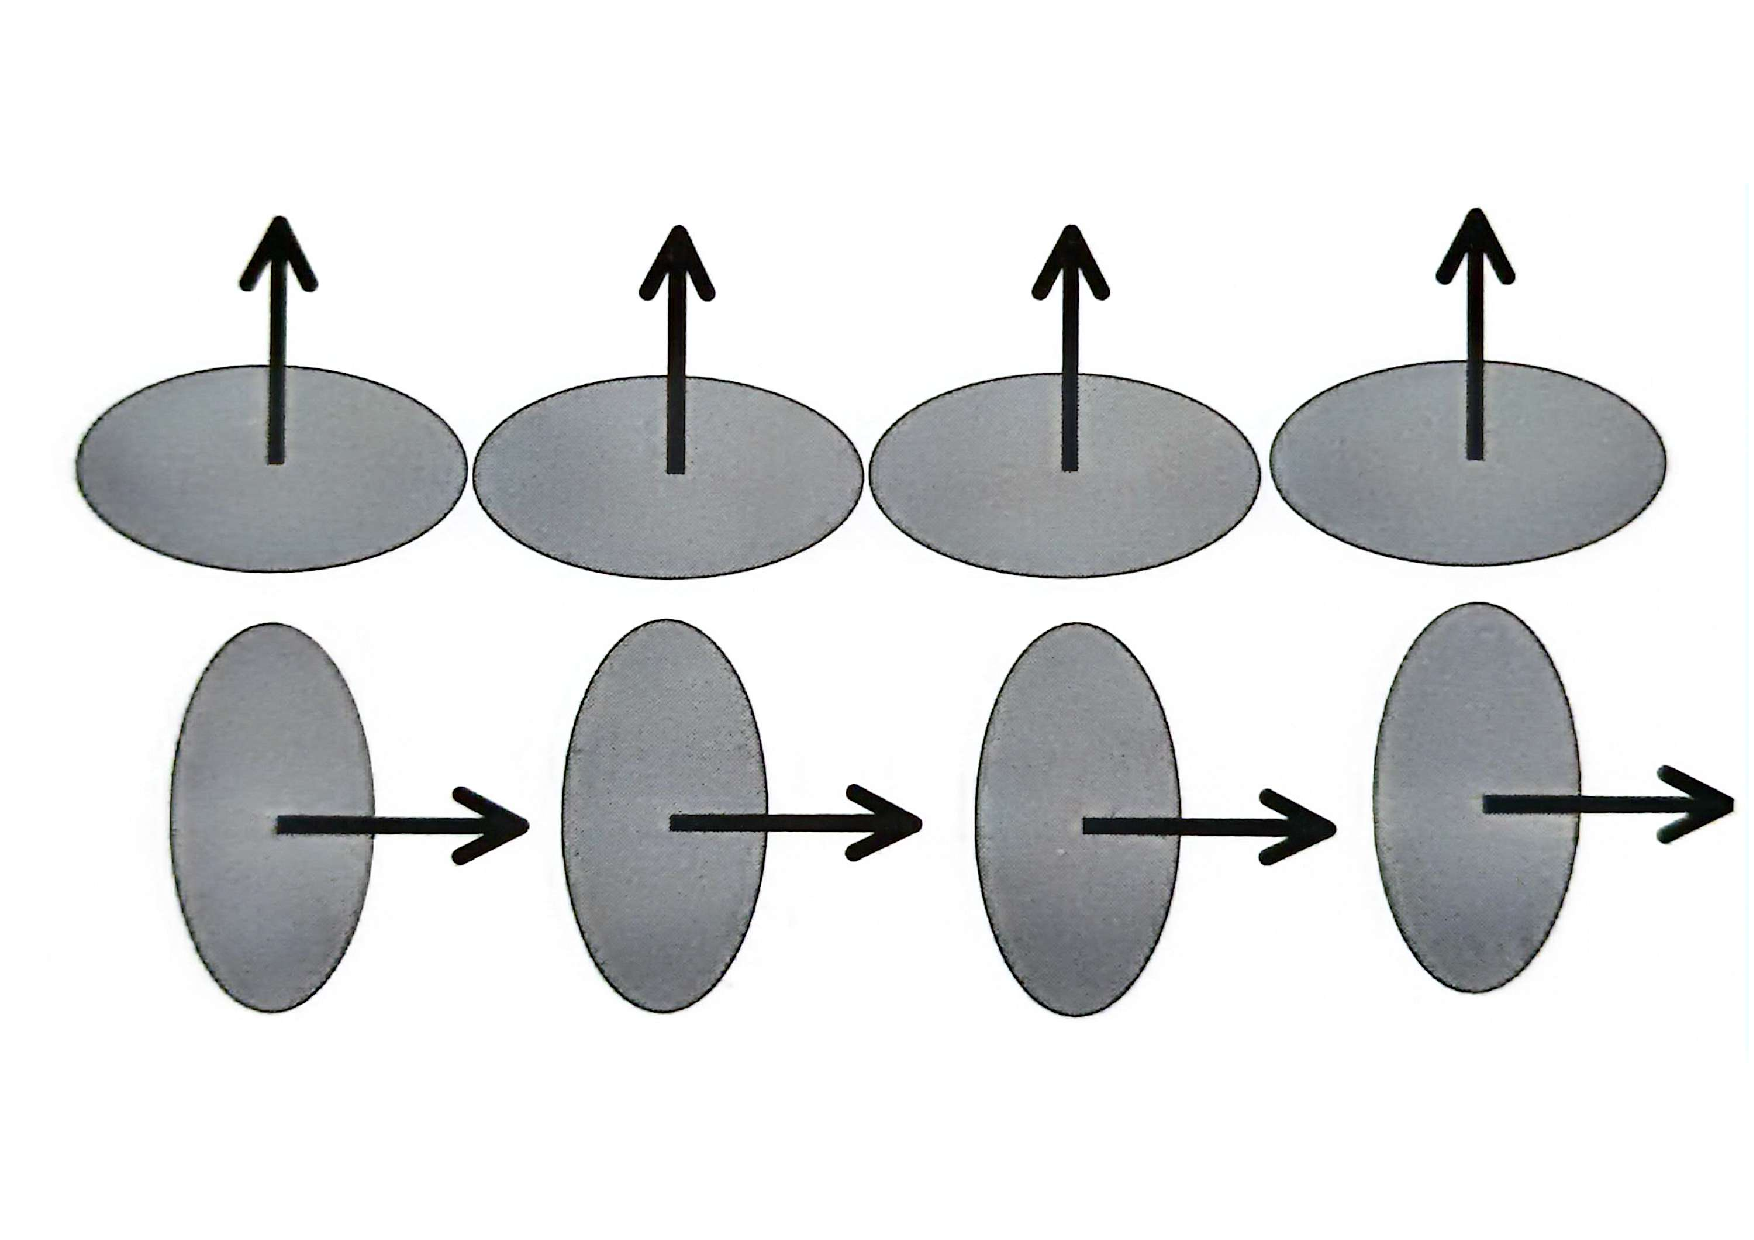
\includegraphics[scale=0.25]{Cuerpo/Ch_10/Fotos libro 6.pdf}
	\caption{Distribución electrónica para diferntes orientaciones del campo mangético aplicado.}
	\label{Fig:10-06}
	\end{figure}
	\item \textbf{Energía de intercambio}. Se determina a partir de 
	
	\begin{equation}
		U = - \sum_{i,j}\Jcal_{ij} \Sn_i \Sn_j
	\end{equation}
	donde la suma se extiende a todos los espines del material. El mínimo de energía de canje en un ferromagnético corresponde de imanación homogénea (todos los espiens alineados).
	\item \textbf{Energía de interacción espín-campo magnético}. Es la energía de interacción de los espines del material ferromagnético con un campo magnético aplicado $\mu_0 \Hn_a$ que viene dado por 
	
	\begin{equation}
		U = - \int \mu_0\Mn \cdot \Hn_a \D V
	\end{equation}
	\item \textbf{Energía magnetostática}. Es debida a la interacción de los dipolos magnéticos con el campo creado por ellos mismos $\Hn_M$:
	
	\begin{equation}
		U = - \int \frac{\mu_0}{2}\Mn \cdot \Hn_M \D V
	\end{equation}
	donde el factor 1/2 se introduce para no contar dos veces la misma interacción. 
	
\end{enumerate}
El mínimo de la energía total no corresponde a la configuración saturada (salvo a altos campos aplicados), sino más bien a cierta estructura de dominios. Las fronteras de separación entre éstos se denominan paredes de Bloch. El cambio de espín ocurre de modo gradual a lo largo de muchas constantes de red (por ejemplo, 300 en el hierro) pues cambios bruscos de espín están penalizados por la contribución de la energía de intercambio. El espesor de la pared Bloch no aumenta, sin embargo, indefinidamente ya que en ella la inmensa mayoría de los espines no están orientados a lo largo del eje de fácil imantación, lo que incrementa su energía. La Fig. \ref{Fig:10-07} muestra cómo aparece la división en dominios de una muestra ferromagnética con objeto de minimizar su energía magnetostática. La subdivisión es frenada tanto por la energía de canje como por la energía de anisotropía.


\begin{figure}[h!] \centering
	\begin{subfigure}{0.45\linewidth} \centering
		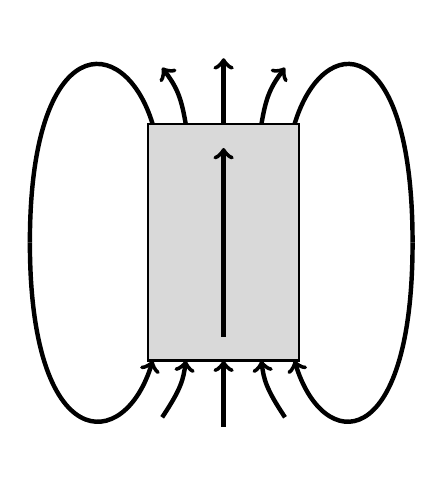
\begin{tikzpicture}[thick,scale=0.6]
			\filldraw[fill=black!15] (0,0)  rectangle (3.2,5);
			\draw[arrows={->},ultra thick] (1.6,0.5)--(1.6,4.5)  ;
			\draw[arrows={->},ultra thick] (1.6,5)--(1.6,6.4)  ;
			\draw[arrows={->},ultra thick] (1.6,-1.4)--(1.6,0)  ;
			
			\draw[arrows={->},ultra thick] (0.8,5) .. controls (0.7,5.6) and (0.6,5.8) .. (0.3,6.2);
			\draw[arrows={->},ultra thick] (2.4,5) .. controls (2.5,5.6) and (2.6,5.8) .. (2.9,6.2);
			
			\draw[arrows={->},ultra thick] (0.3,-1.2) .. controls (0.7,-0.6) and (0.75,-0.4) .. (0.8,0);
			\draw[arrows={->},ultra thick] (2.9,-1.2) .. controls (2.5,-0.6) and (2.45,-0.4) .. (2.4,0);
			
			\draw[ultra thick] (0.1,5) .. controls  (-0.5,7) and  (-2.5,7)   .. (-2.5,2.5);
			\draw[arrows={->},ultra thick] (-2.5,2.5) .. controls   (-2.5,-2) and (-0.5,-2) .. (0.1,0);
			
			\draw[ultra thick] (3.1,5) .. controls  (3.7,7) and  (5.6,7)   .. (5.6,2.5);
			\draw[arrows={->},ultra thick] (5.6,2.5) .. controls   (5.6,-2) and (3.7,-2) .. (3.1,0);
			
		\end{tikzpicture}
		\caption{uniformemente magnetizado.}
		\label{Fig:10-07a}
	\end{subfigure}
	%hspace{-0.2cm}.
	\begin{subfigure}{0.45\linewidth} \centering
		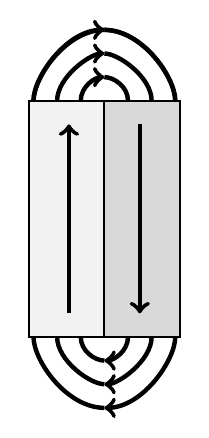
\begin{tikzpicture}[thick,scale=0.6]
			\filldraw[fill=black!5] (-1.6,0) rectangle (1.6,5);
			\draw[arrows={->},ultra thick] (-0.75,0.5)--(-0.75,4.5)  ;
			\filldraw[fill=black!15]  rectangle (1.6,5);
			\draw[,arrows={->},ultra thick] (0.75,4.5)--(0.75,0.5)   ;
			
			
			% Parte de arriba
			\draw[ultra thick] (-1.5,5) .. controls  (-1.5,5.5) and  (-0.8,6.5)   .. (0.0,6.5);
			\draw[ultra thick] (0.0,6.5) .. controls   (0.8,6.5) and  (1.5,5.5) .. (1.5,5);
			
			
			\draw[arrows={->},ultra thick] (-1.5,5) .. controls  (-1.5,5.5) and  (-0.8,6.5)   .. (0.0,6.5);
			\draw[ultra thick] (0.0,6.5) .. controls   (0.8,6.5) and  (1.5,5.5) .. (1.5,5);
			
			\draw[arrows={->},ultra thick] (-1.0,5) .. controls  (-1.0,5.5) and  (-0.3,6)   .. (0.0,6);
			\draw[ultra thick] (0.0,6) .. controls   (0.3,6) and  (1.,5.5) .. (1.,5);
			
			\draw[arrows={->},ultra thick] (-0.5,5) .. controls  (-0.5,5.3) and  (-0.2,5.5)   .. (0.0,5.5);
			\draw[ultra thick] (0.0,5.5) .. controls  (0.2,5.5) and  (0.5,5.3)   .. (0.5,5);
			
			% Parte de abajo
			
			\draw[arrows={->},ultra thick] (1.5,0) .. controls  (1.5,-0.5) and  (0.8,-1.5)   .. (0.0,-1.5);
			\draw[ultra thick] (0,-1.5) .. controls   (-0.8,-1.5) and  (-1.5,-0.5) .. (-1.5,0);
			
			\draw[arrows={->},ultra thick] (1.0,0) .. controls  (1.0,-0.5) and  (0.3,-1)   .. (0.0,-1);
			\draw[ultra thick] (0.0,-1) .. controls   (-0.3,-1) and  (-1.,-0.5) .. (-1.,0);
			
			\draw[arrows={->},ultra thick] (0.5,0) .. controls  (0.5,-0.3) and  (0.2,-0.5)   .. (0.0,-0.5);
			\draw[ultra thick] (0.0,-0.5) .. controls  (-0.2,-0.5) and  (-0.5,-0.3)   .. (-0.5,0);
			
		\end{tikzpicture}
		\caption{dividido en dos dominios.}
		\label{Fig:10-07b}
	\end{subfigure}
	\caption{Aparición de dominios en una muestra ferromagnética. Las flechas indican la orientación de los momentos magnéticos en cada domino.}
	\label{Fig:10-07}
\end{figure}

Bajo la aplicación de un campo, el volumen de los dominios favorablemente orientados crece a costa de aquéllos de peor orientación, y también puede tener lugar la rotación de la imantación de cada dominio (ver Fig. \ref{Fig:10-08}). Este proceso es reversible a bajos campos, pero a mayores campos el desplazamiento de las fronteras de dominios se hace irreversible por la presencia de defectos en la estructura. Debido a esto, si una vez alcanzada la saturación se quita el campo aplicado, se conserva cierta imantación llamada remanente. Para conseguir anular la imantación se debe aplicar un campo en sentido opuesto llamado coercitivo $\mu_0 H_c$. En la figura \ref{Fig:10-09} muestra este fenómeno de la histéresis. Así, como para un núcleo de transformador exigiríamos baja coercitividad para minimizar pérdidas por histéresis, para un imán permanente es conveniente alta coercitividad y remanencia.



\begin{figure}[h!] \centering
	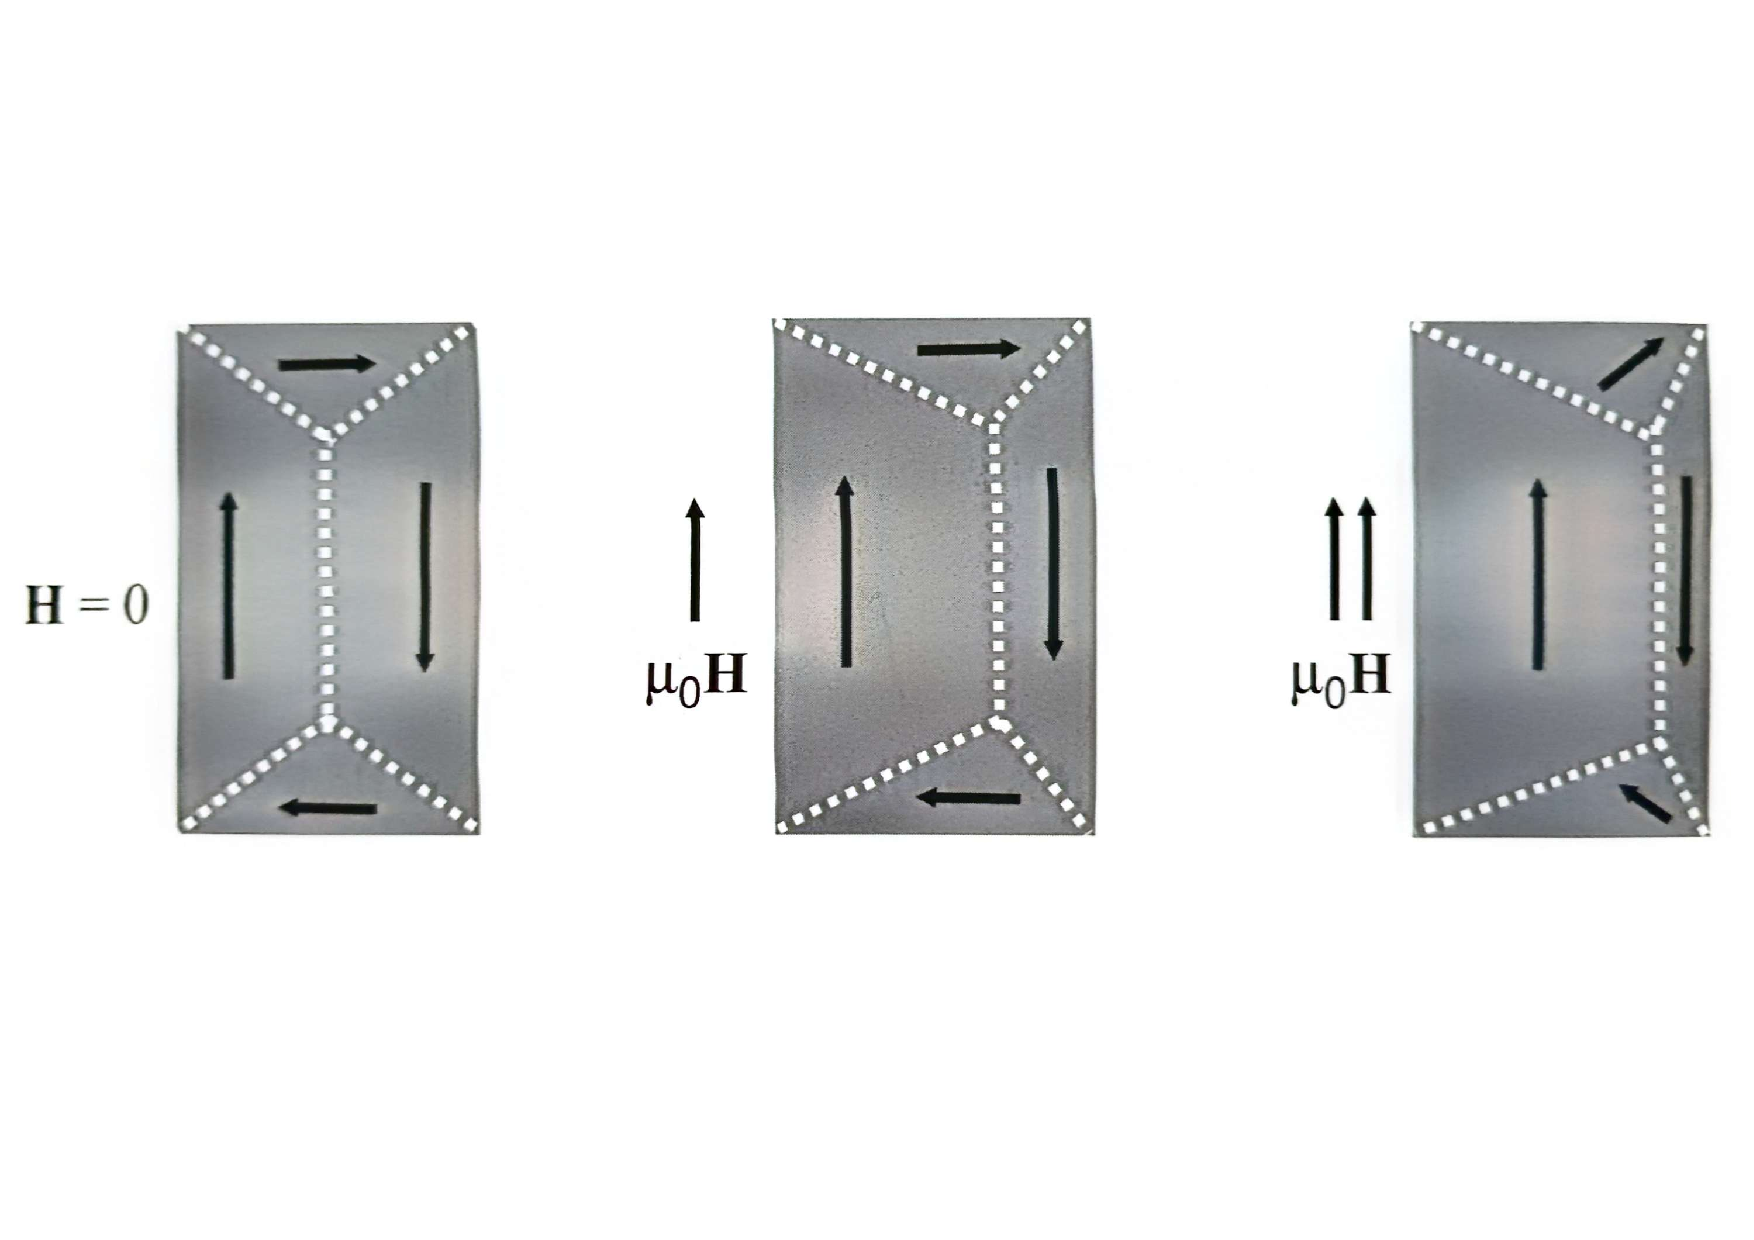
\includegraphics[scale=0.35]{Cuerpo/Ch_10/Fotos libro 8.pdf}
	\caption{Desplazamiento de las fronteras entre dominios debido a una variación del campo magnético aplicado.}
	\label{Fig:10-08}
\end{figure}
\begin{figure}[h!] \centering
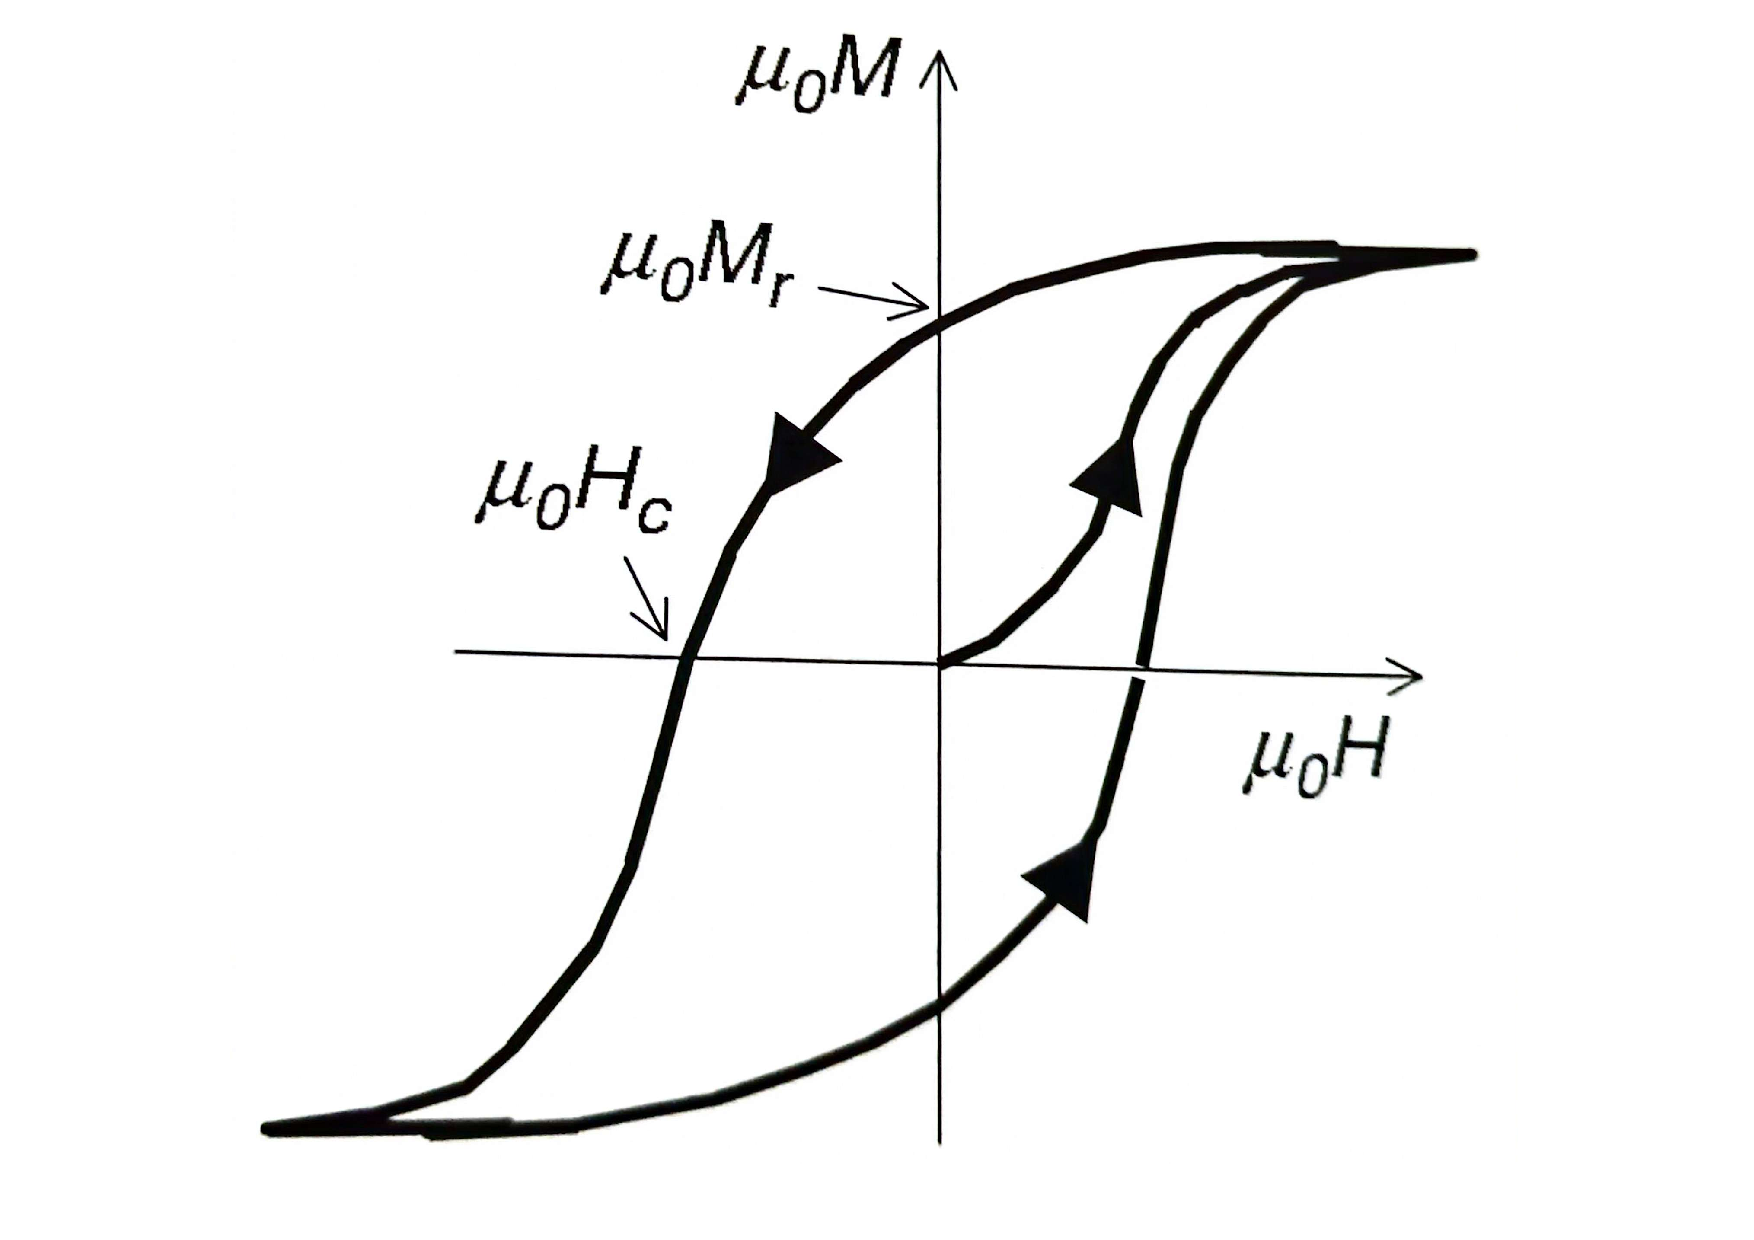
\includegraphics[scale=0.35]{Cuerpo/Ch_10/Fotos libro 9.pdf}
\caption{Histéresis de la dependencia $M(H)$ debida al anclado de las paredes Bloch en los defectos del material.}
\label{Fig:10-09}
\end{figure}
\section{Orden ferrimangnético}

Existe un grupo de materiales que experimentan una interacción de intercambio negativa por la que los momentos magnéticos de espín de los átomos con capas incompletas se orientan antiparalelamente. En este caso el orden magnético se manifiesta por debajo de la llamada \textit{temperatura de Neel}.

Algunos materiales antiferromagnéticos pueden presentar, en su fase ordenada, una magnetización no nula (por ejemplo si los iones que los componen presentan momentos magnéticos distintos). Estos materiales se conocen como \textbf{ferrimagnéticos}. La mayoría de los materiales ferrimagnéticos son cristales iónicos por lo que poseen una baja conductividad eléctrica.
